\documentclass{beamer}
% imprimir
% \documentclass[handout]{beamer} 
% \usepackage{pgfpages}
% \pgfpagesuselayout{4 on 1}[a4paper,landscape,border shrink=5mm]

\mode<presentation> {
  \usetheme{Warsaw}
  \setbeamercovered{transparent}
}

\usebackgroundtemplate{
\includegraphics[width=\paperwidth]{format/libresoft-bg.png}}
\usepackage[spanish]{babel}
\usepackage[utf8]{inputenc}
\usepackage{graphics}
\usepackage{amssymb} % Simbolos matematicos

%\definecolor{libresoftgreen}{RGB}{162,190,43}
%\definecolor{libresoftblue}{RGB}{0,98,143}

%\setbeamercolor{titlelike}{bg=libresoftgreen}

%% Metadatos del PDF.
\hypersetup{  
  pdftitle={Sistemas operativos libres para servidores},
  pdfauthor={Miguel Vidal},
  pdfcreator={GSyC/Libresoft},
  pdfproducer=PDFLaTeX,
  pdfsubject={Curso arquitectura de servidores con software libre},
}
%%

\begin{document}

\title{Sistemas operativos libres para servidores}
\subtitle{Arquitectura de servidores con software libre}
\institute{\{mvidal,jfcastro\}@libresoft.es} 
\author{Miguel Vidal, José Castro}
%\date{\today}
\date{8 de abril de 2011}

\frame{
\maketitle
\begin{center}

\includegraphics[width=6cm]{format/gsyc-urjc}
\end{center}
}

%% License slide
\begin{frame}
  \vspace{2cm}
  \begin{flushright}
    {\footnotesize \copyright{} 2009-2011 Miguel Vidal, Jose Castro.} \\
%    \vspace{0.25cm}
    \medskip
    {\scriptsize Esta presentación se distribuye bajo \\ licencia Creative Commons Reconocimiento 3.0 España}
%    \vspace{0.10cm}
  \end{flushright}
  \begin{center}
    \href{http://creativecommons.org/licenses/by/3.0/es}{
\includegraphics[width=2cm]{format/cc-by.png}} \\
    {\tiny \url{http://creativecommons.org/licenses/by/3.0/es}}
  \end{center}
\end{frame}%%

%%%%%%%%%%%%%%%%%%%%%%%%%%%%%%%%%%%%%%%%%%%%%%%%%%%%%%%%%%%%%%%%%%%%%%%

\begin{frame}
\frametitle{¿Quiénes somos?}

\begin{itemize}
\item \alert{Miguel Vidal} (\url{http://gsyc.es/~mvidal}): 


	\begin{itemize}

\footnotesize

	\item Desplegó la actual infraestructura HA de \href{http://www.morfeo-project.org}{Morfeo} y ha colaborado en la administración y mantenimiento a bajo nivel de la plataforma \href{http://www.osor.eu}{OSO-R}. 
	\item Administró los servidores de barrapunto.com durante seis años.
	\item Coordinador del Máster de Software Libre (URJC) y profesor en la Escuela de Negocios EOI.
	\item Responsable del proyecto de traducción al español de la \href{http://www.openbsd.org/translation.html\#WHO}{documentación de OpenBSD}.
	\end{itemize}

\normalsize

\item \alert{José Castro} (\url{http://gsyc.es/~jfcastro}): 

	\begin{itemize}

\footnotesize

	\item Responsable de sistemas de la plataforma HA de \href{http://www.morfeo-project.org}{Morfeo}. 
	\item Parte del equipo técnico de la plataforma europea \href{http://www.osor.eu}{OSO-R}.
	\item Coordinador de la asignatura de ``Implantación'' en el Máster oficial de software libre de la URJC.
	\item Miembro fundador de Madrid-OSUG (comunidad de usuarios de OpenSolaris en Madrid).
	\end{itemize}

\end{itemize}
\end{frame}

\normalsize

\begin{frame}
  \frametitle{Agenda}

%  \begin{itemize}[<+->]
\begin{enumerate}
\item Breve historia de Unix
\item Variantes de Unix
\end{enumerate}

\end{frame}


%%%%%%%%%%%%%%%%%%%%%%%%%%%%%%%%%%%%%%%%%%%%%%%%%%%%%%%%%%%%%%%%%%%%%%%


\section{Breve historia de Unix}

\begin{frame}
  \begin{center}
    \Huge{Breve historia de Unix}
  \end{center}
\end{frame}

%%%%%%%%%%%%%%%%%%%%%%%%%%%%%%%%%%%%%%%%%%%%%%%%%%%%%%%%%%%%%%%%%%%%%%%


\begin{frame}
\frametitle{¿Qué es Unix?}


\begin{itemize}
\item Sistema operativo multitarea y multiusuario. Muy portable (C). 
\item No hay un solo Unix, sino numerosas ramas. 
\item Probablemente cientos de variantes a lo largo de más de 40 años de historia.
\item Se desarrolla al tiempo que Internet y es la base de la tecnología internet (TCP/IP).
\item Los Unices comparten una estructura común, compatibilidad binaria (ELF), POSIX shell, servicios y utilidades como awk, echo, ed, vi y muchas otras.
\end{itemize}

\end{frame}

%%%%%%%%%%%%%%%%%%%%%%%%%%%%%%%%%%%%%%%%%%%%%%%%%%%%%%%%%%%%%%%%%%%%%%%

\begin{frame}
\frametitle{Universo Unix}


\begin{itemize}
\item \alert{Universo}: nombre con el que tradicionalmente se conocen las variantes y entornos de Unix.
\item Es muy raro que un sysadmin sea responsable de un solo SO.
\item Unix es muy diverso: de móviles a supercomputadoras.
\item Donde más se percibe esta diversidad es en la administración de sistemas.
\end{itemize}

\url{http://en.wikipedia.org/wiki/Universe_(Unix)}

\end{frame}


%%%%%%%%%%%%%%%%%%%%%%%%%%%%%%%%%%%%%%%%%%%%%%%%%%%%%%%%%%%%%%%%%%%%%%%


\begin{frame}
\frametitle{¿Qué es Unix? La marca}


\begin{itemize}
\item Oficialmente Unix es una marca registrada, controlada por el consorcio Open Group: \textsc{UNIX\texttrademark}
\item El Open Group, formado por grandes corporaciones (Oracle, HP, IBM, Fujitsu...) concede el uso de la marca a quienes cumplen con la Single UNIX Specification (SUS), la versión 4 es también conocida como POSIX:2008 (Portable Operating System Interface [for Unix]).
\item El uso de la marca cuesta dinero y solo los Unixes comerciales (y privativos) tienen la certificación: AIX, HP-UX, SCO, Solaris, Mac OS X, IRIX...
\item El certificado no requiere el código fuente, por lo que pueden no tener código en común ni ser derivados del Unix original.
\item Comparten POSIX shell, servicios y utilidades como awk, echo, ed, vi y muchas otras.
\end{itemize}

\end{frame}


%%%%%%%%%%%%%%%%%%%%%%%%%%%%%%%%%%%%%%%%%%%%%%%%%%%%%%%%%%%%%%%%%%%%%%%

\begin{frame}
\frametitle{¿Qué es Unix?}


\begin{itemize}
\item Para los modelos de desarrollo abiertos, la especificación es demasiado cara e insostenible.
\item GNU: \textbf{G}NU's \textbf{N}ot \textbf{U}nix. En la década de 1980 intentó desarrollar un sustituto libre de Unix (junto al kernel Linux es la base de los actuales sistemas GNU/Linux).
\item Para los SOs que no cumplen la especificación, se suele usar el término \textit{Unix-like} (``tipo Unix''), ``*nix'' o ``Un*x'' para sortear el problema del uso de la marca (aunque esto no gusta a sus propietarios).
\item FreeBSD tiene una certificación "C99" (ISO 9899:1999) conforme POSIX, que cumple en gran parte con SUS.
\item Linux usa una especificación LSB (Linux Standard Base), muy próximo a POSIX y que más o menos siguen todas las distribuciones. 
\end{itemize}

\end{frame}

%%%%%%%%%%%%%%%%%%%%%%%%%%%%%%%%%%%%%%%%%%%%%%%%%%%%%%%%%%%%%%%%%%%%%%%

\begin{frame}
\frametitle{Clases de Unix}

Clasificación de Eric Raymond:

\begin{itemize}
\item \alert{Unix genético}: descendientes del código Unix original de AT\&T (muchos Unix comerciales y los actuales BSD).
\item \alert{Unix de marca}: los que tienen la especificación SUS (Solaris, AIX, HP-UX, MacOS X...)
\item \alert{Unix funcional}: los que se acercan a la especificación POSIX o se comportan de forma consistente como Unix (como Linux o Minix), pero no poseen la marca ni descienden del código del Unix original.
\end{itemize}

\end{frame}


%%%%%%%%%%%%%%%%%%%%%%%%%%%%%%%%%%%%%%%%%%%%%%%%%%%%%%%%%%%%%%%%%%%%%%%

\begin{frame}
\frametitle{El surgimiento de Unix}

El nacimiento de Unix fue una auténtica revolución del software:

\begin{itemize}

\item 1969: Ken Thompson inventó Unix (mismo año que Arpanet).
\item Surge de los deshechos de Multics, en AT\&T (Bell Labs). 
\item Dennis Ritchie inventa un nuevo lenguaje llamado C para usarlo en el Unix de Thompson. 
\item Primer sistema operativo portable y modular (KISS), frente a anteriores sistemas incompatibles y costosos.
\item Se extiende rápidamente y de forma no oficial por AT\&T. Y por Arpanet (hardware distinto, gracias a C).
\item Acuerdo judicial (\textit{antitrust}) de 1956 impide a AT\&T comercializar Unix: debe licenciarlo (con fuentes) a quien se lo solicite.

\end{itemize}

\end{frame}

%%%%%%%%%%%%%%%%%%%%%%%%%%%%%%%%%%%%%%%%%%%%%%%%%%%%%%%%%%%%%%%%%%%%%%%

\begin{frame}
\frametitle{Años setenta: Unix y Berkeley}

\begin{itemize}

\item CSRG (Computer Systems Research Group) de Berkeley:
	\begin{itemize}
	\item Importancia de compartir fuentes (cultura Unix ``original'').
	\item Limitado por la licencia AT\&T (poco desde el punto de vista práctico, todos la tenían).
	\item Financiado por DARPA (DoD).
	\item Utilizado por mucho software privativo (SunOS, Ultrix, etc.)
	\end{itemize}

\item Primera Internet:
	\begin{itemize}
	\item Implementaciones de referencia, disponibles para todos: la base de los estándares actuales y servicios actuales.
	\item La Red como herramienta de cooperación (news, ftp, e-mail).
	\item La comunidad de usuarios proporciona el mejor soporte.
	\end{itemize}

\end{itemize}

\end{frame}

%%%%%%%%%%%%%%%%%%%%%%%%%%%%%%%%%%%%%%%%%%%%%%%%%%%%%%%%%%%%%%%%%%%%%%%

\begin{frame}
% \frametitle{Historia de Unix}


\begin{figure}[h]

\begin{center}
  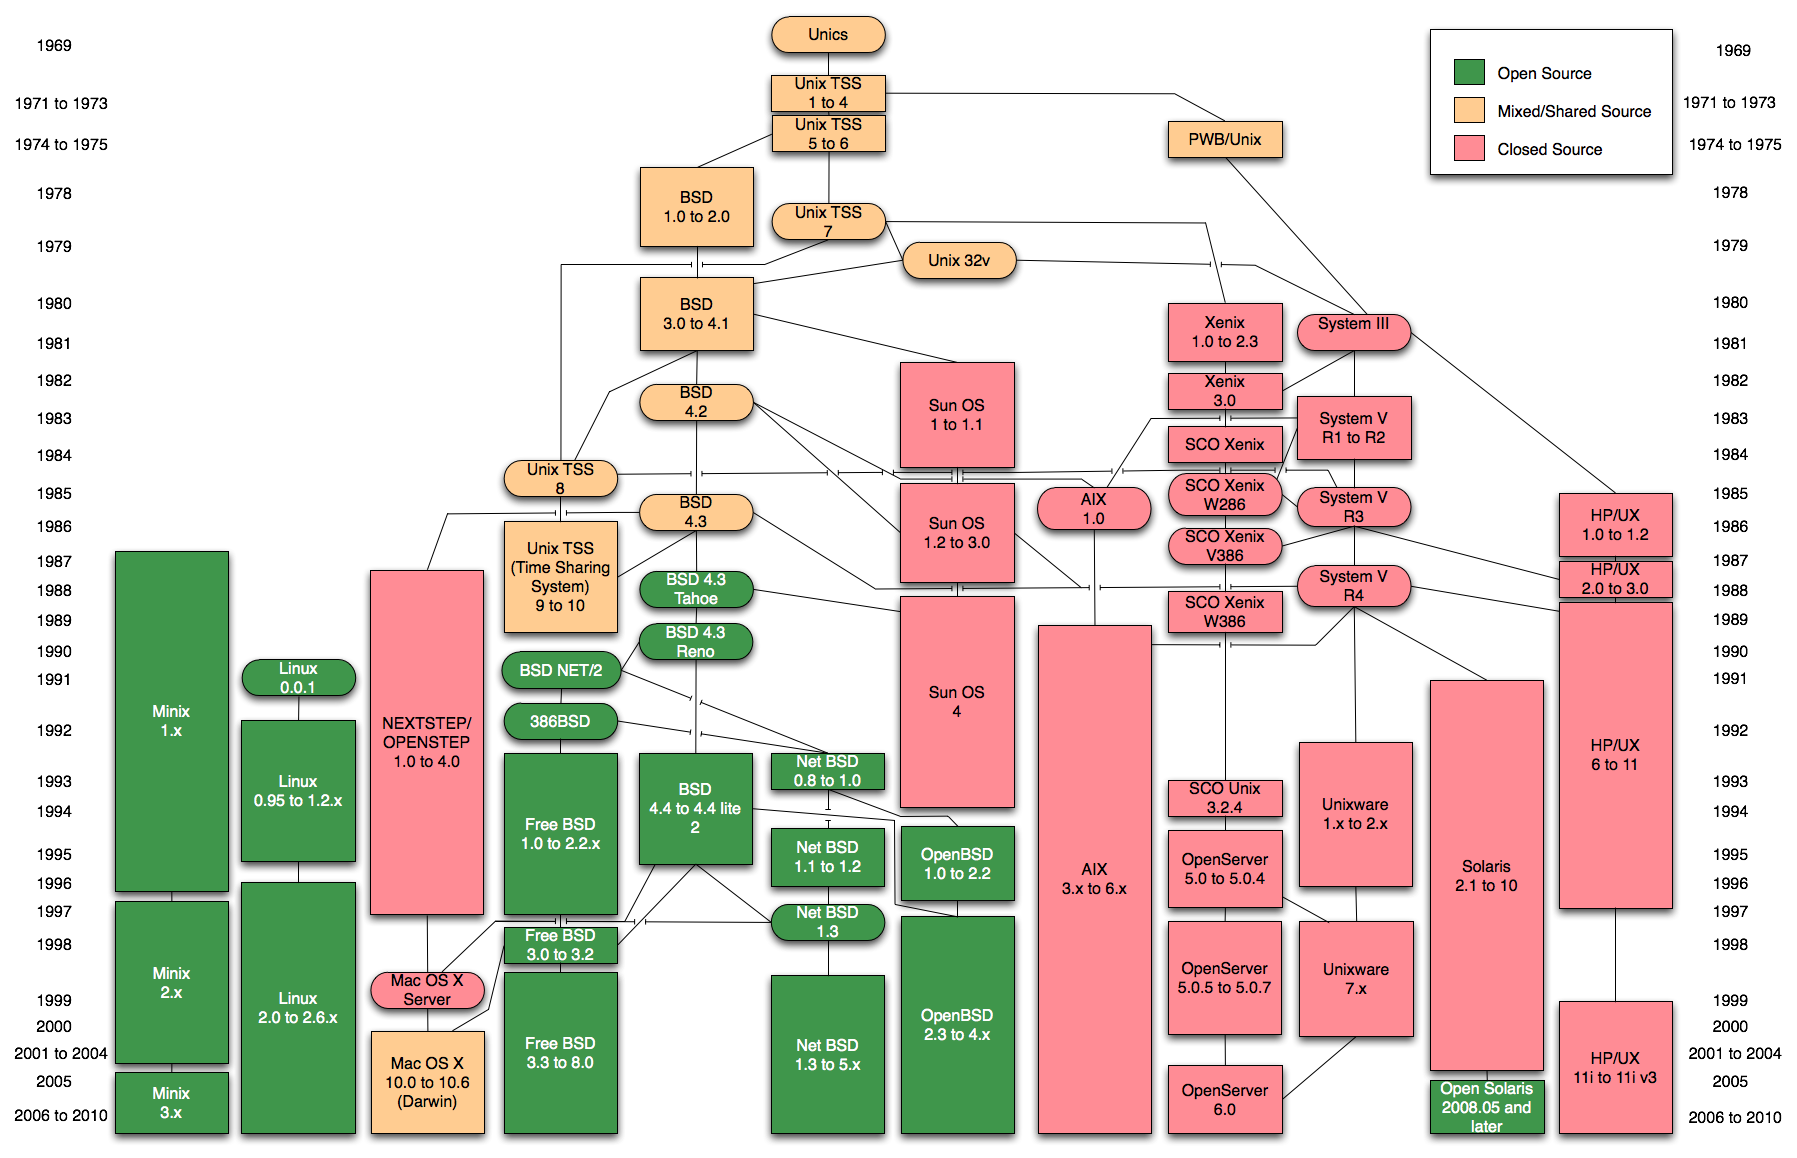
\includegraphics[height=2.7in]{figs/Unix_history-simple.png}
  \caption{{\footnotesize Historia de Unix. \textit{Fuente: Wikipedia}}}
\end{center}
\end{figure}


\end{frame}

%%%%%%%%%%%%%%%%%%%%%%%%%%%%%%%%%%%%%%%%%%%%%%%%%%%%%%%%%%%%%%%%%%%%%%

\begin{frame}
\frametitle{La herencia de BSD}

\begin{itemize}
\item El Computer Systems Research Group (CSRG) libera la implementación de TCP/IP que desarrollaron ellos y todos los SO la adoptan (Net/1, 1989). 
\item Las distribuciones NetBSD, FreeBSD y OpenBSD surgen a partir de la adaptación original de 386BSD, basada en 4.4 BSD-Lite del CSRG (1992).
\item Desde la distribución de 386BSD el desarrollo es rápido y se consigue un sistema estable.
\item Mezcla de bazar y catedral, en paralelo al desarrollo de Linux.
\end{itemize}

\end{frame}

%%%%%%%%%%%%%%%%%%%%%%%%%%%%%%%%%%%%%%%%%%%%%%%%%%%%%%%%%%%%%%%%%%%%%%

\begin{frame}
\frametitle{La ética hacker}

Stephen Levy, en \textit{Hackers: Heroes of the Computer Revolution} (1984), acuña la expresión ``ética hacker'' de forma retrospectiva:

\begin{enumerate}
\item Acceso ilimitado a los ordenadores y a todo aquello que puede enseñarte algo.
\item Toda la información debe ser libre
\item Es necesario promover la descentralización
\item Los hackers no deben ser juzgados por sus títulos académicos, su edad o posición.
\item Se puede crear belleza con una computadora.
\item Los ordenadores pueden cambiar la vida a mejor.
\end{enumerate}

\pause

\begin{center}
\alert{El software libre es el heredero directo de estos principios.}
\end{center}

\end{frame}


%%==================================================================
%%---------------------------------------------------------------

\section{Variantes de Unix}

\begin{frame}
  \begin{center}
    \Huge{Variantes de Unix}
  \end{center}
\end{frame}


%%%%%%%%%%%%%%%%%%%%%%%%%%%%%%%%%%%%%%%%%%%%%%%%%%%%%%%%%%%%%%%%%%%%%%

\begin{frame}
\frametitle{Variantes de Unix}

Dos grandes variantes históricas:

\begin{enumerate}
\item System V
\item BSD
\end{enumerate}

\begin{itemize}
\item Algunos sistemas mantenían las dos versiones en paralelo (con comandos, directorios, páginas \texttt{man} y librerías distintos). A estas variantes se les llamaba \alert{``universos''}.
\item Esta división era problemática a la hora de portar aplicaciones y mantener los sistemas.
\item Cada universo fue adoptando lo mejor del otro. 
\item En 1988, se produce una fusión entre ambas: \alert{System R4}. 
\item Hoy día quedan reminiscencias en algunos sistemas, que tienen un directorio separado con los comandos estilo BSD o System V.
\end{itemize}

\end{frame}

%%%%%%%%%%%%%%%%%%%%%%%%%%%%%%%%%%%%%%%%%%%%%%%%%%%%%%%%%%%%%%%%%%%%%%%

\begin{frame}
\frametitle{Un ejemplo: el comando `\texttt{ps}' en Linux}

\begin{figure}[h]

\begin{center}
  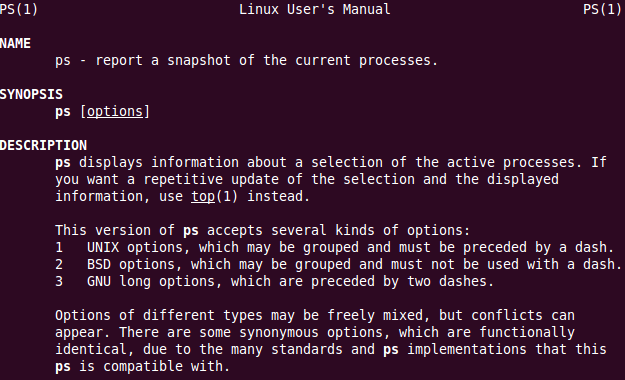
\includegraphics[height=2.0in]{figs/ps.png} \\
  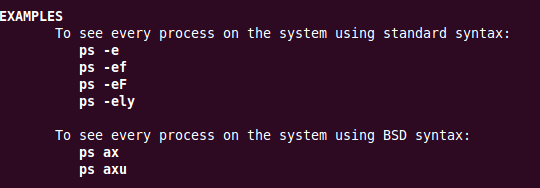
\includegraphics[height=1.0in]{figs/ps-2.png}
%  \caption{{\footnotesize Comando \texttt{ps} en Linux.}}
\end{center}
\end{figure}


\end{frame}


%%%%%%%%%%%%%%%%%%%%%%%%%%%%%%%%%%%%%%%%%%%%%%%%%%%%%%%%%%%%%%%%%%%%%%%

\begin{frame}
\frametitle{Los dos grandes ``universos'' de Unix}


\begin{figure}[h]

\begin{center}
  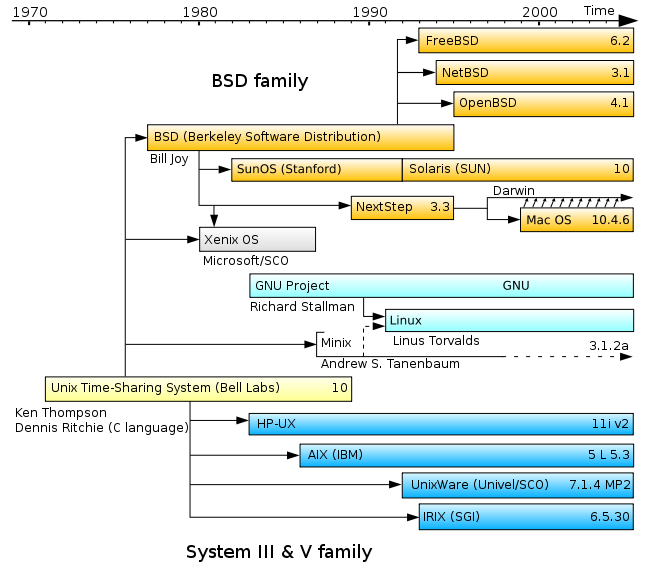
\includegraphics[height=2.55in]{figs/Unix_history.png}
  \caption{{\footnotesize Los dos grandes ``universos'' de Unix. \textit{Fuente: Wikipedia}}}
\end{center}
\end{figure}


\end{frame}


%%%%%%%%%%%%%%%%%%%%%%%%%%%%%%%%%%%%%%%%%%%%%%%%%%%%%%%%%%%%%%%%%%%%%%

\begin{frame}
\frametitle{Unixes libres: los BSD}

No son clones, son derivados del BSD Unix original. Principales proyectos:

\begin{itemize}
\item FreeBSD
\item NetBSD
\item OpenBSD: fork de NetBSD (1995)
\item DragonFly BSD
\item PC-BSD

\end{itemize}

Cada uno tiene, a su vez, numerosas variantes.

\pause

\begin{center}
Lista de SOs basados en BSD: 
\begin{small}
\url{http://en.wikipedia.org/wiki/List_of_BSD_operating_systems}
\end{small}
\end{center}

\end{frame}

%%%%%%%%%%%%%%%%%%%%%%%%%%%%%%%%%%%%%%%%%%%%%%%%%%%%%%%%%%%%%%%%%%%%%%

\begin{frame}
\frametitle{Unixes libres: FreeBSD}

\begin{itemize}
\item Es el BSD más popular. Rápido y optimizado para plataformas i386/amd64.
\item Rápida incorporación de mejoras. 
\item Su kernel incorpora un sistema de virtualización ligera muy apreciado: las \textit{jails}
\item Ha portado el sistema de ficheros ZFS de OpenSolaris.
\end{itemize}

\end{frame}

%%%%%%%%%%%%%%%%%%%%%%%%%%%%%%%%%%%%%%%%%%%%%%%%%%%%%%%%%%%%%%%%%%%%%%

\begin{frame}
\frametitle{Unixes libres: OpenBSD (1)}


\begin{itemize}
\item Se concentra en la corrección, seguridad proactiva, portabilidad (17 arquitecturas) y libertad.
\item Código del sistema base auditado, características de seguridad y criptografía integradas. 
\item PF: el mejor firewall
\item OpenSSH: la mejor shell segura.
\item No intenta estar a la última, prioriza la sencillez y la estabilidad.
\end{itemize}


\end{frame}

%%%%%%%%%%%%%%%%%%%%%%%%%%%%%%%%%%%%%%%%%%%%%%%%%%%%%%%%%%%%%%%%%%%%%%

\begin{frame}
\frametitle{Unixes libres: OpenBSD (y 2)}


\begin{itemize}
\item Comunidad preocupada por la libertad del software: no NDAs, no blobs, la licencia más permisiva de todas (ISC). 
\item La calidad de su documentación es legendaria.
\item Introdujo el uso de CVS y el registro de \textit{commits}, luego adoptado por todas las comunidades de software libre. 
\item Ha logrado que muchos fabricantes de tarjetas de red liberen especificaciones de sus drivers.

\end{itemize}


\end{frame}


%%%%%%%%%%%%%%%%%%%%%%%%%%%%%%%%%%%%%%%%%%%%%%%%%%%%%%%%%%%%%%%%%%%%%%

\begin{frame}
\frametitle{Unixes libres: NetBSD}

\begin{itemize}
\item Orientado a la portabilidad: se propone funcionar en tantas arquitecturas de hardware 
como sea posible (actualmente 57 plataformas distintas).
\item Gracias a su licencia permisiva y su portabilidad, es muy usado en sistemas empotrados.
\item Como todos los BSD actuales, deriva del BSD-lite del CSGR de Berkeley.
\item Es el antecesor de OpenBSD.
\end{itemize}

\end{frame}



%%%%%%%%%%%%%%%%%%%%%%%%%%%%%%%%%%%%%%%%%%%%%%%%%%%%%%%%%%%%%%%%%%%%%%

\begin{frame}
\frametitle{Unixes libres: derivados de OpenSolaris}

Principales proyectos:

\begin{itemize}
\item OpenSolaris
\item illumos
\item Nexenta
\item OpenIndiana
\item SchilliX
\end{itemize}

Todos ellos comparten el kernel SunOS 2.x.

%%%%%%%%%%%%%%%%%%%%%%%%%%%%%%%%%%%%%%%%%%%%%%%%%%%%%%%%%%%%%%%%%%%%%%

\end{frame}

\begin{frame}
\frametitle{OpenSolaris}

\begin{itemize}
\item \alert{Service Manager Facility} (SMF): sistema de gestión de servicios que reemplaza a los scripts init.d (SVR4).
\item \alert{ZFS} (Zettabyte File System): sistema de ficheros nativo de OpenSolaris que provee administración simplificada, cifrado transparente, volúmenes lógicos, snapshots y \textit{copy-on-write}, chequeo de integridad, RAID-Z, NAS/SAN y una escalabilidad inmensa. Bajo licencia CDDL, por tanto no compatible con Linux (hay \textit{workarounds}).
\item \alert{DTrace:} Herramienta de instrumentación para depurar problemas y errores en el SO y sus aplicaciones en producción y en tiempo real, sin apenas impacto.
\end{itemize}

\end{frame}


%%%%%%%%%%%%%%%%%%%%%%%%%%%%%%%%%%%%%%%%%%%%%%%%%%%%%%%%%%%%%%%%%%%%%%%

\begin{frame}
\frametitle{OpenSolaris (2/2)}

\begin{itemize}
\item \alert{Solaris Containers} (aka \alert{Zonas}): virtualización ligera. Entornos aislados con una sola instancia del SO. Equivalente a las \textit{jails} de FreeBSD.
\item \alert{LDOMs}: Paravirtualización para arquitectura Sparc (estilo Xen, pero con las ventajas del soporte multi-hilo de las CPUs Sparc).
\item \alert{Crossbow}: virtualización de redes y recursos para virtualizar el stack completo y las NICs en torno a cualquier servicio. 
\end{itemize}

\end{frame}




%%%%%%%%%%%%%%%%%%%%%%%%%%%%%%%%%%%%%%%%%%%%%%%%%%%%%%%%%%%%%%%%%%%%%%

\begin{frame}
\frametitle{Unixes libres: Linux}

\begin{itemize}
\item Linux es un kernel escrito desde cero. 
\item Es un clon, no un derivado de Unix: pero Dennis Ritchie lo considera un ``Unix de facto''.
\item El proyecto lo inicia Linus Torvalds en 1991, y \textit{just for fun}
\item Incorpora aspectos de las variantes System V y BSD. 
\item Contiene mucho software con origen BSD.
\item Modelo bazar: desde que liberó la primera versión (0.01) se van uniendo cientos de desarrolladores en un esquema innovador (\textit{release early, release often}).
\item Se adopta la licencia GPLv2.
\item Marzo 1994: versión 1.0
\end{itemize}

\end{frame}


%%%%%%%%%%%%%%%%%%%%%%%%%%%%%%%%%%%%%%%%%%%%%%%%%%%%%%%%%%%%%%%%%%%%%%

\begin{frame}
\frametitle{Unixes libres: Linux}

\begin{itemize}

\item Debian y derivados: Ubuntu, Knoppix
\item Red Hat y derivados: RHEL, CentOS, Fedora
\item Gentoo y derivados: Sabayon
\item Ubuntu y derivados: Xubuntu, Kubuntu, Edubuntu, gnewSense, Chrome OS, distros regionales (Guadalinex, LliureX)...
\item Mandriva, SuSE, Slackware...

\end{itemize}

\pause

\begin{center}
Lista de distribuciones Linux: 
\begin{small}
\url{http://en.wikipedia.org/wiki/List_of_Linux_distributions}
\end{small}
\end{center}


\end{frame}

%%%%%%%%%%%%%%%%%%%%%%%%%%%%%%%%%%%%%%%%%%%%%%%%%%%%%%%%%%%%%%%%%%%%%%

\begin{frame}
\frametitle{El caso de MacOS X}

\begin{itemize}

\item En 1997, Apple Computer refunda su sistema operativo a partir de NeXTSTEP. 
\item NeXTSTEP es un SO privativo desarrollado por NeXT a finales de los 80 y primeros 90. 
\item El núcleo del SO está basado en BSD y en el kernel Mach: pasó a llamarse Darwin después de que Apple lo adquiriera. 
\item Darwin es casi todo software libre (Apple Public Source License), pero Mac OS X \alert{NO} lo es.
\item Darwin y Mac OS X son el sistema Unix más usado en el mercado de los sistemas de escritorio. 

\end{itemize}

\end{frame}


%%%%%%%%%%%%%%%%%%%%%%%%%%%%%%%%%%%%%%%%%%%%%%%%%%%%%%%%%%%%%%%%%%%%%%

\begin{frame}
\frametitle{Promiscuidad de los Unixes libres}

Mezclas de proyectos y código \alert{solo} posible con el software libre:

\begin{itemize}

\item Debian kFreeBSD (kernel FreeBSD en Debian)
\item FreeBSD + ZFS
\item Gentoo/*BSD: \textit{userland} GNU manejado por Portage (el árbol de paquetes) con un kernel \{Net,Free,Open\}BSD.
\item Nexenta: Kernel Solaris y \textit{userland} estilo Ubuntu/Debian (paquetes deb, dpkg y apt).

\end{itemize}

\end{frame}

%%%%%%%%%%%%%%%%%%%%%%%%%%%%%%%%%%%%%%%%%%%%%%%%%%%%%%%%%%%%%%%%%%%%%%

\begin{frame}
\frametitle{Consejos a la hora de elegir una versión de Unix}

\begin{itemize}

\item ¿Cuál es el propósito? (no tiene nada que ver un servidor web que un FW)
\item ¿Usas hardware no estándar?
\item ¿Prefieres definir el sistema a tu gusto o buscas un inicio sencillo?
\item ¿Estás interesado en la seguridad?
\item ¿Eres desarrollador? (soportes nativos o extensos para Java, Flash, etc.)
\item ¿Necesitas tecnologías especializadas? (almacenamiento, virtualización...)
\item ¿Tienes requisitos de licencias?

\end{itemize}

\end{frame}

%%%%%%%%%%%%%%%%%%%%%%%%%%%%%%%%%%%%%%%%%%%%%%%%%%%%%%%%%%%%%%%%%%%%%%

\begin{frame}
\frametitle{Distribuciones Unix-like}

\begin{itemize}

\item Familias BSD, Linux y OpenSolaris se dividen en ``distribuciones'' (\textit{aka} ``distros'')
\item Cada ``distro'' es un sistema operativo específico, con diferencias más o menos significativas, con una marca con la que se conoce y se hace \textit{advocacy} o publicidad.
\item Las distros son mantenidas por \textit{desarrolladores}, que pueden ser voluntarios o profesionales, interconectados desde cualquier parte.
\item Suele haber comunidades de usuarios en torno a cada distribución. 
\item Casi siempre están disponibles para descarga.

\end{itemize}

\end{frame}


%%%%%%%%%%%%%%%%%%%%%%%%%%%%%%%%%%%%%%%%%%%%%%%%%%%%%%%%%%%%%%%%%%%%%%

\begin{frame}
\frametitle{Diferencias entre distribuciones}

\begin{itemize}

\item Sistemas de paquetes
\item Hardware soportado
\item Instalador / proceso de instalación
\item Configuración/administración/operación
\item Aplicaciones disponibles
\item Comunidad (tamaño, foco más o menos especializado, etc.)
\item Sistema base homogéneo (BSD) 
\item Esquema de licencias (permisivo vs. copyleft)

\end{itemize}

\end{frame}

%%%%%%%%%%%%%%%%%%%%%%%%%%%%%%%%%%%%%%%%%%%%%%%%%%%%%%%%%%%%%%%%%%%%%%

\begin{frame}
\frametitle{Diferencias entre distribuciones: empaquetado}

\begin{itemize}

\item Sistemas de paquetes de Linux
	\begin{itemize}
	\item \alert{dpkg}: formato original de Debian, portado también a Nexenta/OSol
	\item \alert{apt}: gestor de paquetes .dpkg
	\item \alert{rpm}: formato de RedHat, hoy día portado a muchas distros (incluso a otros Unixes) 
	\item \alert{yum}: gestor de paquetes .rpm
	\item \alert{portage}: Gentoo Linux (portado a FreeBSD)
	\end{itemize}
\end{itemize}

\end{frame}


%%%%%%%%%%%%%%%%%%%%%%%%%%%%%%%%%%%%%%%%%%%%%%%%%%%%%%%%%%%%%%%%%%%%%%

\begin{frame}
\frametitle{Diferencias entre distribuciones: empaquetado}

\begin{itemize}
\item Sistemas de paquetes de BSD
	\begin{itemize}
	\item \alert{pkg/ports} (FreeBSD, OpenBSD)
	\item \alert{pkgsrc} (NetBSD)
	\end{itemize}

\item Sistemas de paquetes de OpenSolaris
	\begin{itemize}
	\item \alert{pkg} (SVR4 package)
	\item \alert{IPS} (aka \alert{pkg(5)}). Soporte ZFS, rollbacks.
	\end{itemize}
\end{itemize}

\end{frame}


%%%%%%%%%%%%%%%%%%%%%%%%%%%%%%%%%%%%%%%%%%%%%%%%%%%%%%%%%%%%%%%%%%%%%%

\begin{frame}
\frametitle{Diferencias entre distribuciones: ports}

\begin{itemize}
	\item Colecciones de ports: FreeBSD y OpenBSD.
	\item Un \texttt{Makefile} descarga los fuentes, las descomprime, parchea, compila y da de alta en la base de datos del sistema de paquetes.
	\item Permiten definir las opciones de compilación 
	\item Muy costoso en tiempo con programas grandes. 
	\item La mayoría de ports tienen paquete precompilado (opción recomendada para OpenBSD)
\end{itemize}

\end{frame}



%%%%%%%%%%%%%%%%%%%%%%%%%%%%%%%%%%%%%%%%%%%%%%%%%%%%%%%%%%%%%%%%%%%%%%

\begin{frame}
\frametitle{Diferencias entre distribuciones: Operación}

Distintas shells por defecto:

\begin{itemize}
\item Linux: \texttt{bash}
\item FreeBSD: \texttt{tcsh} (\texttt{csh} con completado y edición de comandos)
\item OpenSolaris/illumos: \texttt{ksh93} (Korn Shell sde AT\&T, liberada en 2005)
\item OpenBSD: \texttt{pdksh} (Public Domain Korn Shell)
\end{itemize}

\end{frame}

%%%%%%%%%%%%%%%%%%%%%%%%%%%%%%%%%%%%%%%%%%%%%%%%%%%%%%%%%%%%%%%%%%%%%%

\begin{frame}
\frametitle{Diferencias entre distribuciones: scripts de inicio}

\begin{itemize}
\item Unix histórico (Bell Labs): \texttt{/etc/rc} para demonios estándar y \texttt{/etc/rc.local} para demonios añadidos localmente
\item Unix System V de AT\&T: esquema de directorios en \texttt{/etc/rc.d}.
\item \texttt{S-} (start) o \texttt{K-} (kill). Ejemplo: \texttt{S67lpr}
\item Linux: System V con runlevels. Scripts en /etc/init.d, symlinks con S- y K- situados en \texttt{/etc/rc0.d, rc1.d, rc2.d}, etc. que corresponden a los runlevels.
\item BSD mantiene ficheros únicos: /etc/rc.conf y /etc/rc.local 
\item FreeBSD 8: más de 150 ficheros para arrancar demonios en \texttt{/etc/rc.d}.
\item OpenBSD, todo en un fichero único \texttt{/etc/rc.local}. A partir de la versión 4.9, variable \texttt{rc\_scripts} en \texttt{/etc/rc.conf.local}.
\end{itemize}

\end{frame}

%%%%%%%%%%%%%%%%%%%%%%%%%%%%%%%%%%%%%%%%%%%%%%%%%%%%%%%%%%%%%%%%%%%%%%%

\begin{frame}
\frametitle{Scripts de inicio en Linux (System V)}


\begin{figure}[h]

\begin{center}
  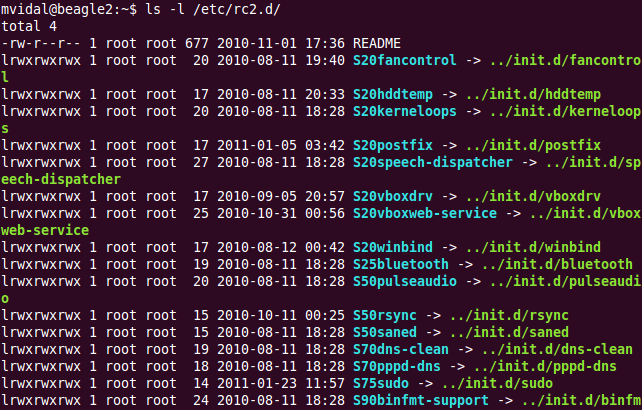
\includegraphics[height=2.7in]{figs/initd.png}
\end{center}
\end{figure}

\end{frame}


%%%%%%%%%%%%%%%%%%%%%%%%%%%%%%%%%%%%%%%%%%%%%%%%%%%%%%%%%%%%%%%%%%%%%%

\begin{frame}
\frametitle{Diferencias entre distribuciones: Licencias}


\begin{itemize}
\item La licencia determina lo que podemos hacer con el software.
\item La distribución (recopilación) puede tener una licencia distinta a los programas por separado, incluso privativa.
\item \alert{Licencias BSD:} 

\begin{itemize}
\item Esquema permisivo y minimalista (BSD, MIT e ISC)
\item 2, 3 y 4 cláusulas. FreeBSD (2-clauses). OpenBSD (ISC)
\item Preserva únicamente los derechos morales (la autoría y el copyright)
\end{itemize}

\item \alert{Licencia Linux} (copyleft): 

\begin{itemize}
\item Kernel y \textit{userland} (GNU) es generalmente copyleft (aunque contiene también herramientas BSD).
\item Si se compila o se combina cualquier cosa con código GPL, el resultado debe ser GPL.
\item Solo si hay redistribución de los cambios, hay que mantener la GPL.
\item Espacio de usuario: cualquier licencia.
\end{itemize}


\end{itemize}

\end{frame}

%%%%%%%%%%%%%%%%%%%%%%%%%%%%%%%%%%%%%%%%%%%%%%%%%%%%%%%%%%%%%%%%%%%%%%


\frame{
\maketitle
\begin{center}

\includegraphics[width=6cm]{format/gsyc-urjc}
\end{center}
}



\end{document}




